\documentclass[12pt, titlepage]{article}

\usepackage[normalem]{ulem}
\usepackage{cancel}
\usepackage[a4paper,margin=1in,footskip=0.25in]{geometry}
\usepackage{indentfirst}
\usepackage[dvipsnames]{xcolor}
\usepackage{tabularx}
\usepackage{booktabs}
\usepackage{hyperref}
\usepackage{listings}
\usepackage{graphicx}
\usepackage{listings}
\usepackage{float}
\hypersetup{
    colorlinks,
    citecolor=black,
    filecolor=black,
    linkcolor=black,
    urlcolor=blue
}
\usepackage[round]{natbib}

%%%%%%%%%%%%%
%%% title %%%
%%%%%%%%%%%%%

\title{\textbf{SE 3XA3: Test Report}\\Lines Per Minute (lpm)}

\author{Team \#16, Lines Per Minute (lpm)\\
Jay Mody - modyj - 400195508\\
Jessica Lim - limj31 - 400173669\\
Maanav Dalal - dalalm1 - 400178115\\
}

\date{\today}

\begin{document}

\maketitle
\begin{table}[hp]
\caption{Revision History} \label{TblRevisionHistory}
\begin{tabularx}{\textwidth}{llX}
\toprule
\textbf{Date} & \textbf{Developer(s)} & \textbf{Change}\\
\midrule
March 27, 2021 & Jay/Jessica/Maanav & Initial document write-up. \\
\midrule
March 30, 2021 & Jay/Jessica/Maanav & Finish test report \\
\bottomrule
\end{tabularx}
\end{table}

\newpage

\maketitle

\pagenumbering{roman}
\tableofcontents
\listoftables
%\listoffigures

\newpage

\pagenumbering{arabic}

\section{Introduction}
This document specifies the results of the testing performed on the lpm package. The document compares the present implementation of lpm to the existing implementation, wpm. It also identifies any changes made to the module as a result of testing, and comments on the testing approaches used. Furthermore, multiple traceability matricies mapping functional requirements to both test cases as well as modules also provided. \\

\section{Requirements Evaluation}
\subsection{Functional Requirements Evaluation}
This section specifies every functional requirement test specified in the Test Plan in a one-to-one mapping. Outputs and test results are documented for every test case. The type of test, initial sate and input and expected output are also included. Further details regarding the individual tests can be found in the Test Plan.\\

%%%% CLI Tests %%%%
\subsubsection{Command Line Interface}

\paragraph{Start Typing Interface}
\begin{enumerate}
\item{\textbf{test-CLI1}: Start Typing Interface\\}
\textbf{Type:} Functional, Manual \\
\textbf{Initial State:} Newly started terminal session.\\
\textbf{Input:} lpm\\
\textbf{Expected output: } The lpm typing interface, all languages should be part of the list of available code snippets.\\
\textbf{Actual Output:} The lpm typing interface, all languages should be part of the list of available code snippets.\\
\textcolor{ForestGreen}{\textbf{Result:} Passed}

\item{\textbf{test-CLI2:} Start the Typing Interface with Specific Languages\\}
\textbf{Type:} Functional, Manual \\
\textbf{Initial State}: Newly started terminal session.\\
\textbf{Input:} lpm python, lpm python java javascript\\
\textbf{Expected output: } The lpm typing interface with only python code snippets, the lpm typing interface with python, java and javascript code snippets\\
\textbf{Actual Output:} The lpm typing interface with only python code snippets, the lpm typing interface with python, java and javascript code snippets\\
\textcolor{ForestGreen}{\textbf{Result:} Passed}
\end{enumerate}

\paragraph{Show Help Menu}

\begin{enumerate}
\item{\textbf{test-CLI3}: Show Help Menu\\}
\textbf{Type:} Functional, Manual\\
\textbf{Initial State:} Terminal session with lpm installed \\
\textbf{Input:} lpm --help \\
\textbf{Expected output: } The text-based help menu.\\
\textbf{Actual Output:} The text-based help menu.\\
\textcolor{ForestGreen}{\textbf{Result:} Passed}
\end{enumerate}

\paragraph{Show Typing Statistics}
\begin{enumerate}

\item{\textbf{test-CLI4}: Show Statistics\\}
\textbf{Type:} Functional, Manual \\
\textbf{Initial State:} Terminal session with lpm installed \\
\textbf{Input:} A. lpm --stats (with existing history) B. lpm --stats (with no history) \\
\textbf{Expected output: }  A. The user's lifetime typing statistics B. Display that there is no history \\
\textbf{Actual Output:} A. The user's lifetime typing statistics B. Display that there is no history \\
\textcolor{ForestGreen}{\textbf{Result:} Passed}

\end{enumerate}

\paragraph{Change Settings}
\begin{enumerate}

\item{\textbf{test-CLI5}: Change Settings\\}
\textbf{Type:} Functional, Manual \\
\textbf{Initial State:} Terminal session with lpm installed \\
\textbf{Input:} lpm --settings \\
\textbf{Expected output: } Open a vim session with lpmconfig.json file in terminal \\
\textbf{Actual Output:} Open a vim session with lpmconfig.json file in terminal \\
\textcolor{ForestGreen}{\textbf{Result:} Passed}

\end{enumerate}

%%%% Typing Editor %%%%
\subsubsection{Typing Editor}

\paragraph{Code Snippet Navigation}
\begin{enumerate}

\item{\textbf{test-TE1}: Display Randomized Order Snippet\\}
\textbf{Type:} Functional, Manual \\
\textbf{Initial State:} Terminal session with lpm installed \\
\textbf{Input:} lpm, lpm \\
\textbf{Expected output: }  Typing interface with random code snippet, Typing interface with random code snippet\\
\textbf{Actual Output:} Typing interface with random code snippet, Typing interface with random code snippet\\
\textcolor{ForestGreen}{\textbf{Result:} Passed}

\item{\textbf{test-TE2}: Next/Prev\\}
\textbf{Type:} Functional, Manual \\
\textbf{Initial State:} Terminal session with lpm installed \\
\textbf{Input:} lpm, then the following combination of arrow keys is pressed: $\rightarrow$, $\leftarrow$, $\leftarrow$, $\rightarrow$\\
\textbf{Expected output: }  The initial code snippet, the next code snippet, the initial code snippet, the previous code snippet, the initial code snippet\\
\textbf{Actual Output:} The initial code snippet, the next code snippet, the initial code snippet, the previous code snippet, the initial code snippet\\
\textbf{Result: } Passed

\item{\textbf{test-TE3}: Start \\}
\textbf{Type:} Functional, Manual \\
\textbf{Initial State:} Terminal session with lpm installed \\
\textbf{Input:} lpm, Type character that is not escape or the arrowkeys \\
\textbf{Expected output: }  Typing interface with started timer \\
\textbf{Actual Output:} Typing interface with started timer \\
\textcolor{ForestGreen}{\textbf{Result:} Passed}

\item{\textbf{test-TE4}: Exit\\}
\textbf{Type:} Functional, Manual \\
\textbf{Initial State:} Terminal session with lpm installed \\
\textbf{Input:} lpm \\
\textbf{Expected output: } Terminal screen exited from lpm \\
\textbf{Actual Output:} Terminal screen exited from lpm \\
\textcolor{ForestGreen}{\textbf{Result:} Passed}

\item{\textbf{test-TE8}: Stop} \\
\textbf{Type:} Functional, Manual \\
\textbf{Initial State:} Terminal session with lpm installed \\
\textbf{Input:} Escape key \\
\textbf{Expected output: } Typing interface with timer ended and cursor at the beginning\\
\textbf{Actual Output:} Typing interface with timer ended and cursor at the beginning\\
\textcolor{ForestGreen}{\textbf{Result:} Passed}
\end{enumerate}

\paragraph{Editor Information}

\begin{enumerate}
\item{\textbf{test-TE5}: Typing Interface Link\\}
\textbf{Type:} Functional, Manual \\
\textbf{Initial State:} Terminal session with lpm installed \\
\textbf{Input:} lpm, then the top link is clicked. \\
\textbf{Expected output: } Typing interface, as well as a link to the hyperlink opened up in the user's browser \\
\textbf{Actual Output:} Typing interface, as well as a link to the hyperlink opened up in the user's browser \\
\textcolor{ForestGreen}{\textbf{Result:} Passed}

\item{\textbf{test-TE6}: Keystroke Information\\}
\textbf{Type:} Functional, Manual \\
\textbf{Initial State:} lpm code snippet in session  \\
\textbf{Input:} A. Key matching next character on screen, B. Key not matching next character on screen\\
\textbf{Expected output: } A. Character in CORRECT\_COLOR B. Character in INCORRECT\_COLOR, All other characters in TEXT\_COLOR  \\
\textbf{Actual Output:} A. Character in CORRECT\_COLOR B. Character in INCORRECT\_COLOR, All other characters in TEXT\_COLOR  \\
\textcolor{ForestGreen}{\textbf{Result:} Passed}

\item{\textbf{test-TE7}: Typing Interface Statistics\\}
\textbf{Type:} Functional, Manual \\
\textbf{Initial State:} Terminal session with lpm installed \\
\textbf{Input:} lpm, then the user presses a character \\
\textbf{Expected output: }Typing interface, with stats information showing \\
\textbf{Actual Output:}  Typing interface \\
\textcolor{ForestGreen}{\textbf{Result:} Passed}

\item{\textbf{test-TE9}: Keystroke Information Correction\\}
\textbf{Type:} Functional, Manual \\
\textbf{Initial State:} lpm session with previously typed characters \\
\textbf{Input:} Backspace key\\
\textbf{Expected output: } Character returned to TEXT\_COLOR and cursor moved back one spot \\
\textbf{Actual Output:} Character returned to TEXT\_COLOR and cursor moved back one spot \\
\textcolor{ForestGreen}{\textbf{Result:} Passed}
\end{enumerate}

%%%% Code Snippets %%%%
\subsubsection{Code Snippets}

\paragraph{Code snippet lengths of valid character and line length}
\begin{enumerate}
\item{\textbf{test-CS1}: Snippet Line Length Test\\}
\textbf{Type:} Functional, Automated \\
\textbf{Initial State:} Snippets object is fully loaded with all lpm code snippets from pickle\\
\textbf{Input:} Every single Snippet stored within the Snippets object \\
\textbf{Expected Output:} Pass or assertion error if any snippet length is larger than MAX\_LENGTH\\
\textbf{Actual Output:} No assertion error raised. Asserts that every snippet length is smaller than MAX\_LENGTH. \\
\textcolor{ForestGreen}{\textbf{Result:} Passed}

\item{\textbf{test-CS2:} Snippet Character Length Test\\}
\textbf{Type:} Functional, Automated \\
\textbf{Initial State:} Snippets object is fully loaded with all lpm code snippets from pickle\\
\textbf{Input:} Every single Snippet stored within the Snippets object \\
\textbf{Expected Output:} Pass or assertion error if any snippet length is larger than MAX\_COLS\\
\textbf{Actual Output:} No assertion error raised. Assertions pass for every individual snippet\\
\textcolor{ForestGreen}{\textbf{Result:} Passed}
\end{enumerate}

\paragraph{Sufficient Code snippets available in Python, Java and Javascript}
\begin{enumerate}

\item{\textbf{test-CS3}: Snippets Per Language} \\
\textbf{Type:} Functional, Automated \\
\textbf{Initial State:} Snippets object is fully loaded with all lpm code snippets from pickle\\
\textbf{Input:} Every single Snippet stored within the Snippets object \\
\textbf{Expected Output:} Pass or assertion error if any language has less than MIN\_SNIPPETS snippets\\
\textbf{Actual Output:} No assertion error raised. Assert all three languages have more than MIX\_SNIPPETS snippets\\
\textcolor{ForestGreen}{\textbf{Result:} Passed}

\end{enumerate}

%%%% Statistics %%%%
\subsubsection{Statistics}

\paragraph{Track statistics per individual code-snippet}
\begin{enumerate}
    \item{\textbf{test-S1}: Test lines per minute speed\\}
    \textbf{Type:} Functional, Dynamic, Automated \\
    \textbf{Initial State:} lpm environment properly setup, Empty stats History\\
    \textbf{Input:} Type one line in 10 seconds, Type 2 lines in 10 seconds, Type zero lines in 10 seconds \\
    \textbf{Expected Output:} 6 lines/min, 12 lines/min, 0 lines/min \\
    \textbf{Actual Output:} For given input, pytest tests assert: 6 lines/min, 12 lines/min, 0 lines/min \\
    \textcolor{ForestGreen}{\textbf{Result:} Passed}

    \item{\textbf{test-S2}: Test characters per minute speed \\}
    \textbf{Type:} Functional, Dynamic, Automated \\
    \textbf{Initial State:} lpm environment properly setup, Empty stats History\\
    \textbf{Input:} Type 20 characters 5 seconds, Type zero characters in 10 seconds\\
    \textbf{Expected Output:} 240 char/min, 0 char/min \\
    \textbf{Actual Output:} For given input, pytest tests assert: 240 char/min, 0 char/min \\
    \textcolor{ForestGreen}{\textbf{Result:} Passed}

    \item{\textbf{test-S3}: Test words per minute speed\\}
    \textbf{Type:} Functional, Dynamic, Automated \\
    \textbf{Initial State:} lpm environment properly setup, Empty stats History\\
    \textbf{Input:} Type 10 words in 10 seconds, Type zero lines in 10 seconds\\
    \textbf{Expected Output:} 60 words/min, 0 words/min \\
    \textbf{Actual Output:} For given input, pytest tests assert: 60 words/min, 0 words/min \\
    \textcolor{ForestGreen}{\textbf{Result:} Passed}

    \item{\textbf{test-S4}: Test errors rate\\}
    \textbf{Type:} Functional, Dynamic, Automated \\
    \textbf{Initial State:} lpm environment properly setup, Empty stats History\\
    \textbf{Input:} Match code statement perfectly, Make one char mistake when typing a 100 char line, Make a mistake on every character\\
    \textbf{Expected Output:} 100\%, 99\%, 0\%\\
    \textbf{Actual Output:} For given input, pytest tests assert: 100\%, 99\%, 0\% \\
    \textcolor{ForestGreen}{\textbf{Result:} Passed}
\end{enumerate}

\paragraph{Track statistics per program lifetime}
\begin{enumerate}
    \item{\textbf{test-S5: Test lines per minute lifetime speed\\}}
    \textbf{Type:} Functional, Dynamic, Automated\\
    \textbf{Initial State:} lpm environment properly setup, clean slate with newly installed program \\
    \textbf{Input:} Type 3 lines in 10 seconds, close session, type 4 lines in 10 seconds \\
    \textbf{Expected Output:} 21 lines per minute \\
    \textbf{Actual Output:} For given input across multiple sessions, pytest tests assert: 12 lines per minute \\
    \textcolor{ForestGreen}{\textbf{Result:} Passed}
\end{enumerate}

%%%%%%%%%%%%%%%%%%%
%%%% NFR Tests %%%%
%%%%%%%%%%%%%%%%%%%
\subsection{Nonfunctional Requirements Evaluation}

This section specifies every non-functional requirement test specified in the Test Plan in a one-to-one mapping. Outputs and test results are documented for every test case. The type of test, initial sate and input and expected output are also included. Further details regarding the individual tests can be found in the Test Plan.\\

\subsubsection{Look and Feel}

\paragraph{The typing interface shall respond to a user input within 10ms.}
\begin{enumerate}
    \item{\textbf{test-LF1: User input latency $\leq$ 10ms testing}\\}
    \textbf{Type:} Manual\\
    \textbf{Initial State:}  lpm is opened and a code snippet is loaded.\\
    \textbf{Input:} User will type out the code snippet\\
    \textbf{Expected output: } The game should perform all functions properly with a max of 10ms latency. \\
    \textbf{Actual Output:} No noticeable latency. \\
    \textcolor{ForestGreen}{\textbf{Result:} Passed}
\end{enumerate}

\paragraph{The user interface should be visible in both light and dark terminal backgrounds.}
\begin{enumerate}
    \item{\textbf{test-LF2: Light theme test}\\}
    \textbf{Type:} Manual\\
    \textbf{Initial State:}  Command line is open\\
    \textbf{Input:} The user launches lpm in light mode\\
    \textbf{Expected output: } The lpm package opens in light mode\\
    \textbf{Actual Output:} The lpm package launched in light mode. \\
    \textcolor{ForestGreen}{\textbf{Result:} Passed}

    \item{\textbf{test-LF3: Dark theme test}\\}
    \textbf{Type:} Manual\\
    \textbf{Initial State:}  Command line is open\\
    \textbf{Input:} The user launches lpm in dark mode\\
    \textbf{Expected output: } The lpm package opens in dark mode\\
    \textbf{Actual Output:} The lpm package launched in dark mode. \\
    \textcolor{ForestGreen}{\textbf{Result:} Passed}
\end{enumerate}

\paragraph{The provided theme shall be easy on the eyes and follow the WCAG AA or AAA
specification in terms of colour choice.}
\begin{enumerate}
    \item{\textbf{test-LF4: WCAG AA testing}\\}
    \textbf{Type:} Manual\\
    \textbf{Initial State:}  lpm is opened and a few characters are typed, such that all potential colours are displayed (i.e. some correct characters as well as some incorrect characters.)\\
    \textbf{Input:} The hex value of all the colours for each theme of the lpm package\\
    \textbf{Expected output: }A WCAG number above 4.5\\
    \textbf{Actual Output:} A WCAG number of 4.7 was achieved. \\
    \textcolor{ForestGreen}{\textbf{Result:} Passed}
\end{enumerate}

\paragraph{The code snippets chosen should be diverse, and representative of the languages’ syntax}
\begin{enumerate}
    \item{\textbf{test-LF5: Code snippet diversity testing}\\}
    \textbf{Type:} Manual\\
    \textbf{Initial State:}  lpm is loaded\\
    \textbf{Input:} The user will use skipping functions to view multiple code snippets.\\
    \textbf{Expected output: } The user will have seen various code snippets and be able to comment on their diversity / uniqueness. \\
    \textbf{Actual Output:} The user commented that there was a variety of logic, functions, imports, lengths, and in general code snippets across languages were unique. \\
    \textcolor{ForestGreen}{\textbf{Result:} Passed}
\end{enumerate}

\paragraph{The entirety of the user interface should fit within a terminal window sized MAX\_COLS (width) x MAX\_LINES (length) or greater}
\begin{enumerate}
    \item{\textbf{test-LF6: lpm resoultion testing}\\}
    \textbf{Type:} Manual\\
    \textbf{Initial State:}  lpm is loaded in a terminal of size MAX\_COLS (width) x MAX\_LINES \\
    \textbf{Input:} The user will type a code snippet\\
    \textbf{Expected output: }  The user will have seen the entirety of the lpm screen, including their code snippet and statistics. Through this process, they will be able to inform us if the package was usable in a window with a resolution of MAX\_COLS (width) x MAX\_LINES \\
    \textbf{Actual Output:} The user commented that the package was usable at resolutions above MAX\_COLS X MAX\_LINES. \\
    \textcolor{ForestGreen}{\textbf{Result:} Passed}
\end{enumerate}

%%%% Usability and Humanity %%%%
\subsubsection{Usability and Humanity}
\paragraph{The system’s typing interface, as well as its cursor indicator, should be intuitive.\\
The system shall be easy to use for anyone with basic knowledge of the console.\\
The instructions will be easily comprehensible by anyone with basic understanding of English.\\}
\begin{enumerate}
\item{\textbf{test-UH1: General use testing}\\}
    \textbf{Type:} Manual\\
    \textbf{Initial State:}  Command line is open\\
    \textbf{Input:} User will open lpm and interact with the software\\
    \textbf{Expected output: }  The user's overall impressions on the usability, typing interface, and comprehensibility of the lpm package \\
    \textbf{Actual Output:} The user commented that the package was overall straightforward and worked as expected. They further commented that instructions were easily comprehended and the package was intuitive to use. \\
    \textcolor{ForestGreen}{\textbf{Result:} Passed}
\end{enumerate}

\paragraph{The user will only require the keys on a typical 60\% keyboard to correctly type all given code.}
\begin{enumerate}
    \item{\textbf{test-UH2: 60\% keyboard testing}\\}
    \textbf{Type:} Manual\\
    \textbf{Initial State:}  lpm is opened and a code snippet is loaded. The user is using a 60\% keyboard\\
    \textbf{Input:} The user types through two code snippets. \\
    \textbf{Expected output: }  The user is either successful or unsuccessful in typing the required code snippets\\
    \textbf{Actual Output:} The user ran into no issues while typing through multiple snippets using lpm, as their 60\% keyboard had all required keys to type snippets contained within lpm. \\
    \textcolor{ForestGreen}{\textbf{Result:} Passed}
\end{enumerate}

%%%% Performance %%%%
\subsubsection{Performance}
\paragraph{When the user loads the package, excluding the first time loading, the time it takes for the package to be ready to accept user input shall not exceed 1 second.}
\begin{enumerate}
    \item{\textbf{test-PF1}\\}
    \textbf{Type:} Manual\\
    \textbf{Initial State: } Command line is open, lpm package previous loaded\\
    \textbf{Input:} lpm command is entered\\
    \textbf{Expected output: } the lpm package is interactive \\
    \textbf{Actual Output:} the lpm package is interactive \\
    \textcolor{ForestGreen}{\textbf{Result:} Passed}
\end{enumerate}

\paragraph{Application should be available 99.999\% (5 nines) of the time. This translates
to 5.26 minutes of downtime in a given year, afforded by user updates of python or lpm,
as well as unforeseen circumstances in the CI/CD Pipeline.}
\begin{enumerate}
    \item{\textbf{test-PF2}\\}
    \textbf{Type:} Manual\\
    \textbf{Initial State:} PyPI page opened\\
    \textbf{Input:} python package name, 'lpm'\\
    \textbf{Expected output: } Uptime based on pypi statistics and versioning\\
    \textbf{Actual Output:} lpm was always available to the user unless they were updating the package. \\
    \textcolor{ForestGreen}{\textbf{Result:} Passed}
\end{enumerate}

%%%% Operational and Environmental %%%%
\subsubsection{Operational and Environmental}
\paragraph{The system shall work on Python 3.6 and up}
\begin{enumerate}
    \item{\textbf{test-OE1}\\}
    \textbf{Type:} Manual\\
    \textbf{Initial State:} Python 3.6 or above, lpm repository installed\\
    \textbf{Input:} run lpm\\
    \textbf{Expected output: } Package is successfully run on multiple versions of Python. \\
    \textbf{Actual Output:} Package was tested on Python 3.6.0, 3.7.5, and 3.8.1 and no errors or differences were recorded between versions. \\
    \textcolor{ForestGreen}{\textbf{Result:} Passed}
\end{enumerate}

\paragraph{The system shall work on Linux, macOS, and Windows operating systems.}
\begin{enumerate}
    \item{\textbf{test-OE2}\\}
    \textbf{Type:} Manual\\
    \textbf{Initial State:} lpm repository installed\\
    \textbf{Input:} run lpm, run CI/CD test suite\\
    \textbf{Expected output: } lpm can be installed and run on all 3 platforms. \\
    \textbf{Actual Output:} lpm was installed and successfully run on Ubuntu 18.04, Windows 10, and MacOS 11. \\
    \textcolor{ForestGreen}{\textbf{Result:} Passed}
\end{enumerate}

\paragraph{In terms of computer specs, the package shall run on any computer that is
able to run Python 3 based on their respective minimum requirements (i.e.
if running on Python 3, the user’s computer shall at least have Python 3’s minimum
requirements to be supported officially by the lpm package).}
\begin{enumerate}
    \item{\textbf{test-OE3}\\}
    \textbf{Type:} Manual\\
    \textbf{Initial State:} A third party who uses a laptop that is 10 years old does not currently have lpm installed opens their terminal.\\
    \textbf{Input:} The third party types pip install lpm, runs lpm, then types out one code snippet\\
    \textbf{Expected output: }  Qualitative information on the performance of lpm, and information about whether it matched their standards.\\
    \textbf{Actual Output:} lpm was run and performed very similarly to on a newer device - latency was low, and performance did not suffer. \\
    \textcolor{ForestGreen}{\textbf{Result:} Passed}
\end{enumerate}

\paragraph{Application should be installable via the pip package manager.}
\begin{enumerate}
    \item{\textbf{test-OE4}\\}
    \textbf{Type:} Manual\\
    \textbf{Initial State:} Environment without lpm package installed\\
    \textbf{Input:} pip install --upgrade lpm\\
    \textbf{Expected output: } lpm package successfully updated.\\
    \textbf{Actual Output:} lpm package successfully updated.\\
    \textcolor{ForestGreen}{\textbf{Result:} Passed}
\end{enumerate}

%%%% Maintainability and Support %%%%
\subsubsection{Maintainability and Support}
\paragraph{Application should be easy to update (via pip)}
\begin{enumerate}
    \item{\textbf{test-MS1}\\}
    \textbf{Type:} Manual\\
    \textbf{Initial State:} Environment with non-current version of lpm installed\\
    \textbf{Input:} Changes are committed, and a pull request is made for an issue.\\
    \textbf{Expected output: } Pull request is accepted, and changes are merged into the master branch. The lpm package now has the changes\\
    \textbf{Actual Output:} Pull request is accepted, and changes are merged into the master branch. The lpm package now has the changes\\
    \textcolor{ForestGreen}{\textbf{Result:} Passed}
\end{enumerate}

\paragraph{ It should be easy to add additional code snippets.}
\begin{enumerate}
    \item{\textbf{test-MS2}\\}
    \textbf{Type:} Manual\\
    \textbf{Initial State:} lpm installed\\
    \textbf{Input:} New code snippet can be added with a permalink. A pull request is made requesting addition of the snippet.\\
    \textbf{Expected output: } The code snippet is added to the lpm repository and shipped to users in the next release of lpm. Users will get new snippets when they reset snippets\\
    \textbf{Actual Output:}  The code snippet is added to the lpm repository and shipped to users in the next release of lpm. Users will get new snippets when they reset snippets\\
    \textcolor{ForestGreen}{\textbf{Result:} Passed}
\end{enumerate}

%%%% Security %%%%
\subsubsection{Security}
\paragraph{External systems shall not have access to the system.}
\begin{enumerate}
    \item{\textbf{test-SC1}\\}
    \textbf{Type:} Manual\\
    \textbf{Initial State:} lpm is installed on the system \\
    \textbf{Input:} A third party tries to access the system without access to it.\\
    \textbf{Expected output: } The party is unable to access it since there are 0 states in which someone external can access \\
    \textbf{Actual Output:}  The party is unable to access it since there are 0 states in which someone external can access \\
    \textcolor{ForestGreen}{\textbf{Result: } Passed}
\end{enumerate}

%%%% Security %%%%
\subsubsection{Cultural}
\paragraph{Code snippets that include harmful, vulgar, controversial, political, or offensive
content shall not be displayed in lpm}
\begin{enumerate}
    \item{\textbf{test-CT1}\\}
    \textbf{Type:} Manual\\
    \textbf{Initial State:} lpm is installed and running.\\
    \textbf{Input:} A third party will page through all of the quotes in the lpm tool.\\
    \textbf{Expected output:} The third party will inform us if they find any of the snippets harmful, vulgar, controversial, political, or offensive, and if so, corrective measures will be taken in the form of removing said quotes from the document. \\
    \textbf{Actual Output:}  No harmful, vulgar, controversial, political, or offensive code snippets were found throughout the entirety of our code snippets database. \\
    \textcolor{ForestGreen}{\textbf{Result:} Passed}
\end{enumerate}

%%%% Legal %%%%
\subsubsection{Legal}
\paragraph{Code snippets shall have a valid open source license or the developers have given explicit permission} to be displayed in lpm
\begin{enumerate}
    \item{\textbf{test-LG1}\\}
    \textbf{Type:} Manual\\
    \textbf{Initial State:} lpm repository \\
    \textbf{Input:} A code snippet is added to the repository with link to code snippet \\
    \textbf{Expected Output:} Each code snippet provides a link to a source repository. The link either comes from a repository with an open source license, or lpm has explicit permissions from the developer.\\
    \textbf{Actual Output:} Each code snippet provides a link to a source repository. The link either comes from a repository with an open source license, or lpm has explicit permissions from the developer.\\
    \textcolor{ForestGreen}{\textbf{Result:} Passed}
\end{enumerate}

\begin{table}[H]
    \centering
    \begin{tabular}{|c|c|}
\hline
\multicolumn{2}{|c|}{Tests results} \\ \hline
Test ID \# & Pass-Fail \\ \hline
test-CLI1 & \textcolor{ForestGreen}{passed} \\ \hline
test-CLI2 & \textcolor{ForestGreen}{passed} \\ \hline
test-CLI3 & \textcolor{ForestGreen}{passed} \\ \hline
test-CLI4 & \textcolor{ForestGreen}{passed} \\ \hline
test-CLI5 & \textcolor{ForestGreen}{passed} \\ \hline
test-TE1 & \textcolor{ForestGreen}{passed} \\ \hline
test-TE2 & \textcolor{ForestGreen}{passed} \\ \hline
test-TE3 & \textcolor{ForestGreen}{passed} \\ \hline
test-TE4 & \textcolor{ForestGreen}{passed} \\ \hline
test-TE5 & \textcolor{ForestGreen}{passed} \\ \hline
test-TE6 & \textcolor{ForestGreen}{passed} \\ \hline
test-TE7 & \textcolor{ForestGreen}{passed} \\ \hline
test-TE8 & \textcolor{ForestGreen}{passed} \\ \hline
test-TE9 & \textcolor{ForestGreen}{passed} \\ \hline
test-CS1 & \textcolor{ForestGreen}{passed} \\ \hline
test-CS2 & \textcolor{ForestGreen}{passed} \\ \hline
test-CS3 & \textcolor{ForestGreen}{passed} \\ \hline
test-S1 & \textcolor{ForestGreen}{passed} \\ \hline
test-S2 & \textcolor{ForestGreen}{passed} \\ \hline
test-S3 & \textcolor{ForestGreen}{passed} \\ \hline
test-S4 & \textcolor{ForestGreen}{passed} \\ \hline
test-S5 & \textcolor{ForestGreen}{passed} \\ \hline
test-LF1 & \textcolor{ForestGreen}{passed} \\ \hline
test-LF2 & \textcolor{ForestGreen}{passed} \\ \hline
test-LF3 & \textcolor{ForestGreen}{passed} \\ \hline
test-LF4 & \textcolor{ForestGreen}{passed} \\ \hline
test-LF5 & \textcolor{ForestGreen}{passed} \\ \hline
test-LF6 & \textcolor{ForestGreen}{passed} \\ \hline
test-UH1 & \textcolor{ForestGreen}{passed} \\ \hline
test-UH2 & \textcolor{ForestGreen}{passed} \\ \hline
test-PF1 & \textcolor{ForestGreen}{passed} \\ \hline
test-PF2 & \textcolor{ForestGreen}{passed} \\ \hline
test-OE1 & \textcolor{ForestGreen}{passed} \\ \hline
test-OE2 & \textcolor{ForestGreen}{passed} \\ \hline
test-OE3 & \textcolor{ForestGreen}{passed} \\ \hline
test-OE4 & \textcolor{ForestGreen}{passed} \\ \hline
test-MS1 & \textcolor{ForestGreen}{passed} \\ \hline
test-MS2 & \textcolor{ForestGreen}{passed} \\ \hline
test-SC1 & \textcolor{ForestGreen}{passed} \\ \hline
test-CT1 & \textcolor{ForestGreen}{passed} \\ \hline
test-LG1 & \textcolor{ForestGreen}{passed} \\ \hline
\end{tabular}
    \caption{Tests results}
    \label{tab:nfrtrace}
\end{table}

\newpage
\section{Comparison to Existing Implementation}
Our implementation adds many changes to the existing implementation (wpm). For instance, the way that modules interacted with eachother - namely between the Game, Screen, and Stats modules. These changes helped to improve the property of maintainability, as we followed the separation of concerns principle in a better fashion than the initial implementation did. This change also improved the ease of testing, as in the initial implementation, the Game module and the Stats module both calculated user typing statistics, which would have required us to validate both calculations in our testing. In contrast, we ensured that only the Stats module was doing any calculations, and the Game Module acted solely as a controller. These changes also resulted in improvements to the readability of the code for future changes. Other things that have changed in contrast with the existing implementation consist of: Implementing the ability to interpret code snippets, an 'LPM' metric, as well as the ability to choose between different types of snippets (in this case, we segmented using language). \\

In terms of testing, the wpm testing framework (based on our review of the repository) only has test for importing of quotes (the equivalent of code snippets on lpm). In comparison, our test suite is much more comprehensive. Lpm's testing framework covers more modules - including tests for the game, screen and stats modules, which are not tested in wpm. The lpm testing plan also includes manual testing. As a result, it has a code coverage of over 90\%, which is a far greater amount of testing than the wpm package's 6 unit tests.

\section{Unit Testing}
{\color{red}TODO}
Due to the nature of the Scrabble program, where the bag and rack of the player are random and the types of input are non-deterministic, it was infeasible to conduct unit testing for the majority of the modules. Because the majority of the program was tested through the front-end interface in Tkinter, most testing was exploratory testing where the aim was to cover the majority of situations that would occur in regular Scrabble gameplay (for example, placing a word that created more words). For more information regarding the back-end during execution of the moves during a playthrough, print statements to the terminal were used and evaluated after each test. During development, unit testing was conducted on modules in the Model classes, so Bag.py, Rack.py, Board.py, Player.py and Tiles.py. This was conducted with PyTest and was prior to developing the back-end for the Scrabble game to ensure it was correct before connecting it with the front-end. After the front-end to back-end implementation was complete the majority of testing was manual testing through the front-end.

\section{Changes Due to Testing}

\subsection{Functional Requirements Changes Evaluation}
Success and failures traced to Functional Requirements incredibly important when evaluating lpm, and changes were made to the code base when functional requirements. \\

Initially, the automated test-CS3 was failing due to an insufficient amount of Java Python and Javascript snippets. This test brought attention to the fact that requirements were unsatisfied, and prompted the addition of further snippets. \\

The importance of differentiating the function of the ESCAPE key when typing a snippet, compared to when browsing through the snippets, became clear when performing tests test-TE4 and test-TE8. Using the expected inputs and outputs of the test, lpm's game logic was altered so that the functionality matched the requirements. \\

Furthermore, the typeface used for the INCORRRECT\_COLOR was changes due to a test failure in test-TE6. Initially, when character spaces were typed incorrectly, this did not register on the screen. To improve upon the requirement that correct, incorrect, and untyped characters must appear uniquely to the user, a change was made to create a red background for incorrectly typed characters, allowing test-TE6 to pass. \\

\subsection{Look and Feel Changes Evaluation}
Due to test-LF6, a change was made to the resolution size requirements. The MAX\_COLS and MAX\_LINES went outside of the allocated terminal dimensions, so after testing, the resolution sizes were altered appropriately to allow for universal scalability.

\subsection{Usability and Humanity Changes Evaluation}
There were no overall changes made to the code due to tests in the Usability category.

\subsection{Performance Changes Evaluation}
There were no overall changes made to the code due to tests in the Performance category.

\subsection{Operational and Environmental Changes Evaluation}
Due to unit testing, it was decided that Python2 compatibility would not be included for the initial version of lpm as the environments resulted in too many complications. No other changes were made to the user interface due to tests in the Operational and Environmental category.

\subsection{Maintainability and Support Changes Evaluation}

To satisfy test-MS2, changes were made to the code base to simplify the process of adding code snippets. While the original plan was to create JSON objects that would house the properties and links for all open-source code snippets, this proved to be a burden, making it difficult to satisfy test-MS3. To make the process simpler, the data was stored using pickle, which allows users to simply add the url link of a github snippet, making it easier to add additional code snippets.

\subsection{Security Changes Evaluation}
There were no overall changes made to the code due to tests in the Security category.

\subsection{Cultural Changes Evaluation}
There were no overall changes made to the code due to tests in the Cultural category.

\subsection{Legal Changes Evaluation}
There were no overall changes made to the code due to tests in the Legal category.

\section{Automated Testing}
Automated Testing for the lpm package was completed using the pytest testing framework. Given that this is the industry standard for testing in the Python language, it was the ideal choice for testing our program. Automated testing was performed on a per-module basis for the Snippets, Config, and Stats modules. These modules were perfect candidates for automated testing, as they had very low coupling with the other modules, and could be used independently from the application as a whole. However, modules like Screen and Game had higher coupling and proved difficult to unit test. As such, we utilized manual testing in place of automated testing for many of our tests where it made the most sense. Since these manual tests would be utilizing the system as a whole, the automated testing allowed us to be confident that if an error was revealed during testing, it was not a result of the modules that were tested with pytest. \\

The following tests were performed in an automated fashion: test-CS1, test-CS2, test-CS3, test-S1, test-S2, test-S3, test-S4, test-S5. In total, our test plan includes 8 automated tests, however, we ended up implementing an additional 4 tests (giving us a total of 12 automated tests). All 12 tests passed. A picture of the test results is attached below: \\

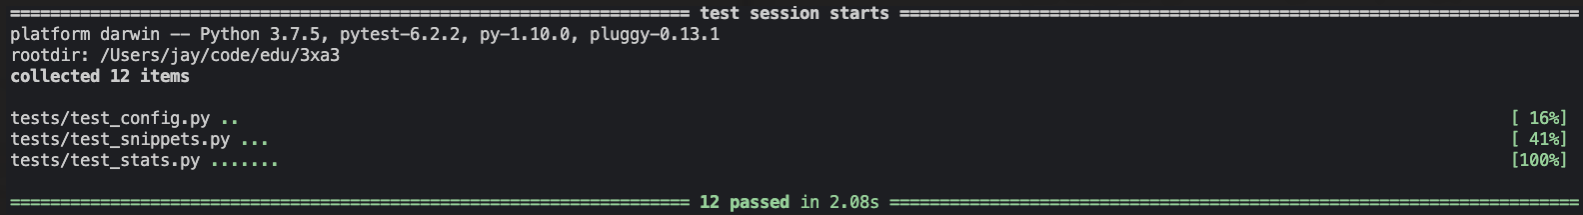
\includegraphics[width=\textwidth]{testResults.png}



\newpage
\section{Trace to Requirements}

The following section displays updated traceability matrices between both functional and nonfunctional requirements to test cases. These were originally outlined in the SRS.

\subsection{Traceability Between Test Cases and Requirements}

\begin{table}[H]
    \centering
\begin{tabular}{|c|c|}
\hline
\multicolumn{2}{|c|}{Functional Requirement Traceability Matrix} \\ \hline
Functional Requirement \# & Test ID \\ \hline
FR1 & test-CLI1 \\ \hline
FR2 & test-CLI1 \\ \hline
FR3 & test-CLI2 \\ \hline
FR4 & test-CLI3 \\ \hline
FR5 & test-CLI4 \\ \hline
FR6 & test-CLI5 \\ \hline
FR7 & test-TE1, test-CLI2 \\ \hline
FR8 & test-TE1 \\ \hline
FR9 & test-TE5 \\ \hline
FR11 & test-TE7 \\ \hline
FR12 & test-TE2 \\ \hline
FR13 & test-TE2 \\ \hline
FR14 & test-TE3 \\ \hline
FR15 & test-TE8 \\ \hline
FR16 & test-TE6 \\ \hline
FR17 & test-TE6 \\ \hline
FR18 & test-TE6 \\ \hline
FR19 & test-TE6, test-TE9 \\ \hline
FR20 & test-TE4 \\ \hline
FR21 & test-CS1 \\ \hline
FR22 & test-CS2 \\ \hline
FR23 & test-CS3 \\ \hline
FR24 & test-CS3 \\ \hline
FR25 & test-S1, test-S5 \\ \hline
FR26 & test-S3, test-S5 \\ \hline
FR27 & test-S2, test-S5 \\ \hline
FR28 & test-S4, test-S5 \\  \hline
\end{tabular}
    \caption{Functional Requirements Traceability Matrix}
    \label{tab:frtrace}
\end{table}

\begin{table}[H]
    \centering
    \begin{tabular}{|c|c|}
\hline
\multicolumn{2}{|c|}{Non-Functional Requirements Traceability Matrix} \\ \hline
Non-Functional Requirement \# & Test ID \\ \hline
NFR1 & test-LF1 \\ \hline
NFR2 & test-LF2, test-LF3 \\ \hline
NFR3 & test-LF4 \\ \hline
NFR4 & test-LF5 \\ \hline
NFR5 & test-LF6 \\ \hline
NFR6 & test-UH1 \\ \hline
NFR7 & test-UH1 \\ \hline
NFR8 & test-UH1 \\ \hline
NFR9 & test-UH2 \\ \hline
NFR10 & test-PF1 \\ \hline
NFR11 & test-PF2 \\ \hline
NFR12 & test-OE1 \\ \hline
NFR13 & test-OE2 \\ \hline
NFR14 & test-OE3 \\ \hline
NFR15 & test-OE4 \\ \hline
NFR16 & test-MS1 \\ \hline
NFR17 & test-MS2 \\ \hline
NFR18 & test-SC1 \\ \hline
NFR19 & test-CT1 \\ \hline
NFR20 & test-LG1 \\ \hline
\end{tabular}
    \caption{Non-Functional Requirements Traceability Matrix}
    \label{tab:nfrtrace}
\end{table}




\newpage
\section{Trace to Modules}

This section displays the traceability matrix between the test cases and the modules. While all function requirements trace to a module, some NFRs are system wide and do not directly trace to a module. \\

The modules of our system are as follows: \\

\begin{table}[H]
    \centering
\begin{tabular}{|p{0.2\textwidth}|p{0.3\textwidth}|p{0.3\textwidth}|}
\hline
\multicolumn{3}{|c|}{Module Traceability Matrix} \\ \hline
Module \# & FR Test ID & NFR Test ID \\ \hline
M1 & test-CLI2, test-CLI3, test-CLI4, test-CLI5 & \\ \hline
M2 & test-CLI5 & \\ \hline
M3 & test-TE1, test-TE2, test-TE3, test-TE4, test-TE8, test-TE6, test-TE9 & test-LF1, test-UH1, test-UH2 \\ \hline
M4 & test-TE1, test-TE2, test-TE3, test-TE4, test-TE8, test-TE5, test-TE6, test-TE7, test-TE9 & test-LF1, test-LF2, test-LF3, test-LF4, test-LF6 \\ \hline
M5 & test-CLI2, test-TE1, test-TE2, test-TE3, test-TE4, test-TE8, test-TE5, test-CS1, test-CS2, test-CS3 & test-LF5, test-MS2, test-CT1, test-LG1\\ \hline
M6 &  test-CLI4, test-TE7, test-S1, test-S2, test-S3, test-S4, test-S5 & \\ \hline
M7 & test-CLI1 & test-PF1\\ \hline
\end{tabular}
    \caption{Module to Test Case Traceability Matrix}
    \label{tab:nfrtrace}
\end{table}




\section{Code Coverage Metrics}

Using \href{https://coverage.readthedocs.io/en/coverage-5.5}{coverage.py}, we found that our combined code coverage across both manual and automated testing was 92\% (see Figure \ref{fig:coverage}). Automated testing by itself was only 23\% (see Figure \ref{fig:cov_auto}). This is expected, as only the Config, Snippets, and Stats modules are included in automated testing. During testing, the code coverage reports helped us uncover several areas that lacked testing, for which we went back and added tests fo. However, there were some tests that we didn't end up implementing due to time constraints. \\

For example, our final code coverage report reveals that a piece of logic in game.py that accounts for snippets with empty lines was never run during testing (see Figure \ref{fig:cov_game}). This was just unlucky, as lpm gives code snippets at random, and the testers happened to have tested snippets that did not contain empty lines. To combat this, we would want to add more test cases which should include a more diverse range of code snippets. \\

Another example would be in the Screen module, for which we did not have test cases for small terminal sizes (see Figure \ref{fig:cov_screen}). To account for this, we would add additional test cases to test-LF6 where the terminal size is insufficient and we expect the program to throw an error informing the user that their terminal is too small.

\begin{figure}[H]
\centering
    \begin{lstlisting}
            Name                 Stmts   Miss  Cover
            ----------------------------------------
            lpm/__init__.py          2      0   100%
            lpm/__main__.py          3      0   100%
            lpm/commandline.py      90     12    87%
            lpm/config.py           28      3    89%
            lpm/game.py            134     15    89%
            lpm/screen.py          146      8    95%
            lpm/snippets.py         63      2    97%
            lpm/stats.py            73      5    93%
            ----------------------------------------
            TOTAL                  539     45    92%
    \end{lstlisting}
    \caption{Coverage for Automated + Manual Testing}
    \label{fig:coverage}
\end{figure}

\begin{figure}[H]
\centering
    \begin{lstlisting}
            Name                 Stmts   Miss  Cover
            ----------------------------------------
            lpm/__init__.py          2      0   100%
            lpm/__main__.py          3      3     0%
            lpm/commandline.py      90     90     0%
            lpm/config.py           28      1    96%
            lpm/game.py            134    134     0%
            lpm/screen.py          146    146     0%
            lpm/snippets.py         63     33    48%
            lpm/stats.py            73      9    88%
            ----------------------------------------
            TOTAL                  539    416    23%
    \end{lstlisting}
    \caption{Coverage for Automated Testing}
    \label{fig:cov_auto}
\end{figure}

\begin{figure}[H]
    \centering
    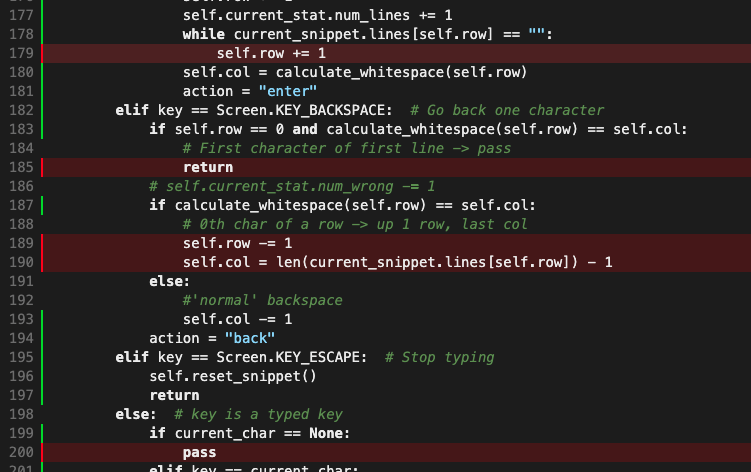
\includegraphics[width=\textwidth]{cov_game.png}
    \caption{Missed coverage for game.py}
    \label{fig:cov_game}
\end{figure}

\begin{figure}[H]
    \centering
    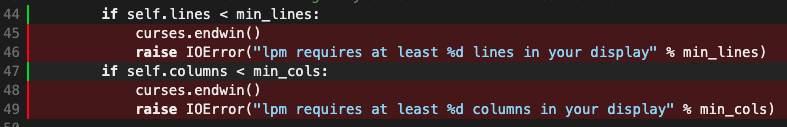
\includegraphics[width=\textwidth]{cov_screen.png}
    \caption{Missed coverage for screen.py}
    \label{fig:cov_screen}
\end{figure}

\end{document}
